% Created by tikzDevice version 0.10.1 on 2017-10-23 14:01:28
% !TEX encoding = UTF-8 Unicode
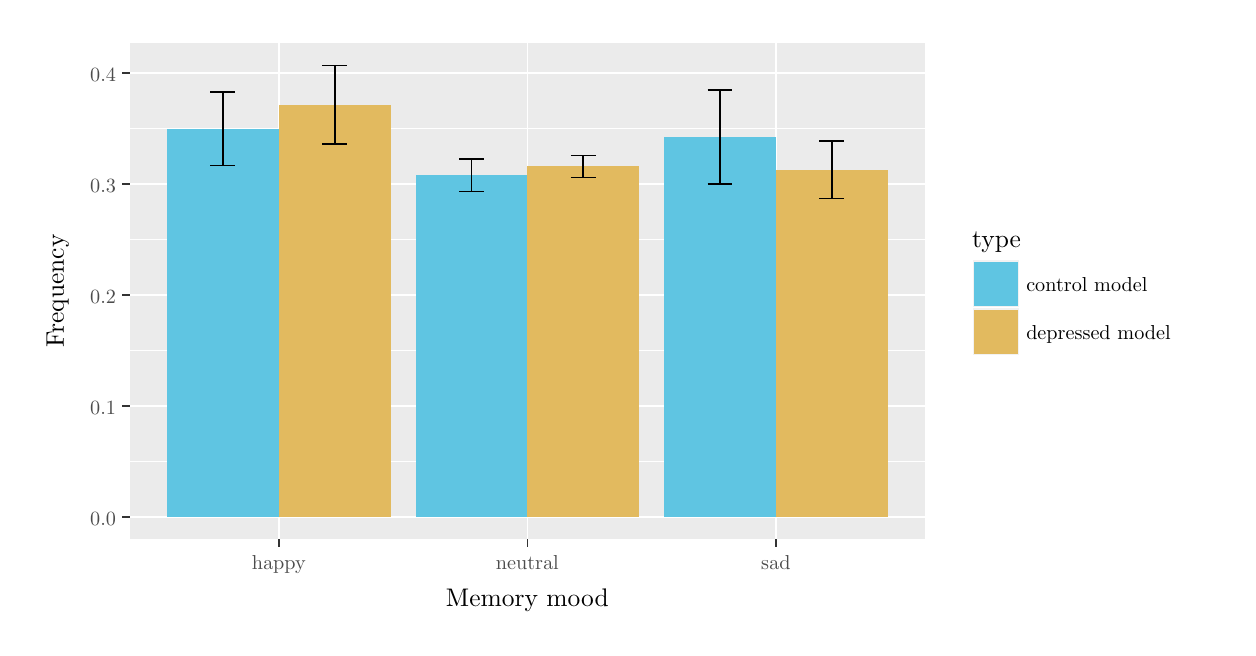
\begin{tikzpicture}[x=1pt,y=1pt]
\definecolor{fillColor}{RGB}{255,255,255}
\path[use as bounding box,fill=fillColor,fill opacity=0.00] (0,0) rectangle (433.62,216.81);
\begin{scope}
\path[clip] (  0.00,  0.00) rectangle (433.62,216.81);
\definecolor{drawColor}{RGB}{255,255,255}
\definecolor{fillColor}{RGB}{255,255,255}

\path[draw=drawColor,line width= 0.6pt,line join=round,line cap=round,fill=fillColor] ( -0.00,  0.00) rectangle (433.62,216.81);
\end{scope}
\begin{scope}
\path[clip] ( 36.87, 31.92) rectangle (324.25,211.31);
\definecolor{fillColor}{gray}{0.92}

\path[fill=fillColor] ( 36.87, 31.92) rectangle (324.25,211.31);
\definecolor{drawColor}{RGB}{255,255,255}

\path[draw=drawColor,line width= 0.3pt,line join=round] ( 36.87, 60.11) --
	(324.25, 60.11);

\path[draw=drawColor,line width= 0.3pt,line join=round] ( 36.87,100.20) --
	(324.25,100.20);

\path[draw=drawColor,line width= 0.3pt,line join=round] ( 36.87,140.28) --
	(324.25,140.28);

\path[draw=drawColor,line width= 0.3pt,line join=round] ( 36.87,180.36) --
	(324.25,180.36);

\path[draw=drawColor,line width= 0.6pt,line join=round] ( 36.87, 40.07) --
	(324.25, 40.07);

\path[draw=drawColor,line width= 0.6pt,line join=round] ( 36.87, 80.16) --
	(324.25, 80.16);

\path[draw=drawColor,line width= 0.6pt,line join=round] ( 36.87,120.24) --
	(324.25,120.24);

\path[draw=drawColor,line width= 0.6pt,line join=round] ( 36.87,160.32) --
	(324.25,160.32);

\path[draw=drawColor,line width= 0.6pt,line join=round] ( 36.87,200.40) --
	(324.25,200.40);

\path[draw=drawColor,line width= 0.6pt,line join=round] ( 90.75, 31.92) --
	( 90.75,211.31);

\path[draw=drawColor,line width= 0.6pt,line join=round] (180.56, 31.92) --
	(180.56,211.31);

\path[draw=drawColor,line width= 0.6pt,line join=round] (270.37, 31.92) --
	(270.37,211.31);
\definecolor{fillColor}{RGB}{226,186,95}

\path[fill=fillColor] ( 90.75, 40.07) rectangle (131.16,188.91);
\definecolor{fillColor}{RGB}{95,197,226}

\path[fill=fillColor] ( 50.34, 40.07) rectangle ( 90.75,180.29);
\definecolor{fillColor}{RGB}{226,186,95}

\path[fill=fillColor] (180.56, 40.07) rectangle (220.97,166.65);
\definecolor{fillColor}{RGB}{95,197,226}

\path[fill=fillColor] (140.15, 40.07) rectangle (180.56,163.53);
\definecolor{fillColor}{RGB}{226,186,95}

\path[fill=fillColor] (270.37, 40.07) rectangle (310.78,165.48);
\definecolor{fillColor}{RGB}{95,197,226}

\path[fill=fillColor] (229.95, 40.07) rectangle (270.37,177.22);
\definecolor{drawColor}{RGB}{0,0,0}

\path[draw=drawColor,line width= 0.6pt,line join=round] (106.47,203.16) --
	(115.45,203.16);

\path[draw=drawColor,line width= 0.6pt,line join=round] (110.96,203.16) --
	(110.96,174.66);

\path[draw=drawColor,line width= 0.6pt,line join=round] (106.47,174.66) --
	(115.45,174.66);

\path[draw=drawColor,line width= 0.6pt,line join=round] ( 66.05,193.61) --
	( 75.03,193.61);

\path[draw=drawColor,line width= 0.6pt,line join=round] ( 70.54,193.61) --
	( 70.54,166.96);

\path[draw=drawColor,line width= 0.6pt,line join=round] ( 66.05,166.96) --
	( 75.03,166.96);

\path[draw=drawColor,line width= 0.6pt,line join=round] (196.28,170.61) --
	(205.26,170.61);

\path[draw=drawColor,line width= 0.6pt,line join=round] (200.77,170.61) --
	(200.77,162.70);

\path[draw=drawColor,line width= 0.6pt,line join=round] (196.28,162.70) --
	(205.26,162.70);

\path[draw=drawColor,line width= 0.6pt,line join=round] (155.86,169.41) --
	(164.84,169.41);

\path[draw=drawColor,line width= 0.6pt,line join=round] (160.35,169.41) --
	(160.35,157.66);

\path[draw=drawColor,line width= 0.6pt,line join=round] (155.86,157.66) --
	(164.84,157.66);

\path[draw=drawColor,line width= 0.6pt,line join=round] (286.08,175.92) --
	(295.07,175.92);

\path[draw=drawColor,line width= 0.6pt,line join=round] (290.57,175.92) --
	(290.57,155.03);

\path[draw=drawColor,line width= 0.6pt,line join=round] (286.08,155.03) --
	(295.07,155.03);

\path[draw=drawColor,line width= 0.6pt,line join=round] (245.67,194.18) --
	(254.65,194.18);

\path[draw=drawColor,line width= 0.6pt,line join=round] (250.16,194.18) --
	(250.16,160.26);

\path[draw=drawColor,line width= 0.6pt,line join=round] (245.67,160.26) --
	(254.65,160.26);
\end{scope}
\begin{scope}
\path[clip] (  0.00,  0.00) rectangle (433.62,216.81);
\definecolor{drawColor}{gray}{0.30}

\node[text=drawColor,anchor=base east,inner sep=0pt, outer sep=0pt, scale=  0.73] at ( 31.92, 37.04) {0.0};

\node[text=drawColor,anchor=base east,inner sep=0pt, outer sep=0pt, scale=  0.73] at ( 31.92, 77.13) {0.1};

\node[text=drawColor,anchor=base east,inner sep=0pt, outer sep=0pt, scale=  0.73] at ( 31.92,117.21) {0.2};

\node[text=drawColor,anchor=base east,inner sep=0pt, outer sep=0pt, scale=  0.73] at ( 31.92,157.29) {0.3};

\node[text=drawColor,anchor=base east,inner sep=0pt, outer sep=0pt, scale=  0.73] at ( 31.92,197.37) {0.4};
\end{scope}
\begin{scope}
\path[clip] (  0.00,  0.00) rectangle (433.62,216.81);
\definecolor{drawColor}{gray}{0.20}

\path[draw=drawColor,line width= 0.6pt,line join=round] ( 34.12, 40.07) --
	( 36.87, 40.07);

\path[draw=drawColor,line width= 0.6pt,line join=round] ( 34.12, 80.16) --
	( 36.87, 80.16);

\path[draw=drawColor,line width= 0.6pt,line join=round] ( 34.12,120.24) --
	( 36.87,120.24);

\path[draw=drawColor,line width= 0.6pt,line join=round] ( 34.12,160.32) --
	( 36.87,160.32);

\path[draw=drawColor,line width= 0.6pt,line join=round] ( 34.12,200.40) --
	( 36.87,200.40);
\end{scope}
\begin{scope}
\path[clip] (  0.00,  0.00) rectangle (433.62,216.81);
\definecolor{drawColor}{gray}{0.20}

\path[draw=drawColor,line width= 0.6pt,line join=round] ( 90.75, 29.17) --
	( 90.75, 31.92);

\path[draw=drawColor,line width= 0.6pt,line join=round] (180.56, 29.17) --
	(180.56, 31.92);

\path[draw=drawColor,line width= 0.6pt,line join=round] (270.37, 29.17) --
	(270.37, 31.92);
\end{scope}
\begin{scope}
\path[clip] (  0.00,  0.00) rectangle (433.62,216.81);
\definecolor{drawColor}{gray}{0.30}

\node[text=drawColor,anchor=base,inner sep=0pt, outer sep=0pt, scale=  0.73] at ( 90.75, 20.91) {happy};

\node[text=drawColor,anchor=base,inner sep=0pt, outer sep=0pt, scale=  0.73] at (180.56, 20.91) {neutral};

\node[text=drawColor,anchor=base,inner sep=0pt, outer sep=0pt, scale=  0.73] at (270.37, 20.91) {sad};
\end{scope}
\begin{scope}
\path[clip] (  0.00,  0.00) rectangle (433.62,216.81);
\definecolor{drawColor}{RGB}{0,0,0}

\node[text=drawColor,anchor=base,inner sep=0pt, outer sep=0pt, scale=  0.92] at (180.56,  7.83) {Memory mood};
\end{scope}
\begin{scope}
\path[clip] (  0.00,  0.00) rectangle (433.62,216.81);
\definecolor{drawColor}{RGB}{0,0,0}

\node[text=drawColor,rotate= 90.00,anchor=base,inner sep=0pt, outer sep=0pt, scale=  0.92] at ( 13.08,121.61) {Frequency};
\end{scope}
\begin{scope}
\path[clip] (  0.00,  0.00) rectangle (433.62,216.81);
\definecolor{fillColor}{RGB}{255,255,255}

\path[fill=fillColor] (335.63, 92.62) rectangle (428.12,150.61);
\end{scope}
\begin{scope}
\path[clip] (  0.00,  0.00) rectangle (433.62,216.81);
\definecolor{drawColor}{RGB}{0,0,0}

\node[text=drawColor,anchor=base west,inner sep=0pt, outer sep=0pt, scale=  0.92] at (341.32,137.34) {type};
\end{scope}
\begin{scope}
\path[clip] (  0.00,  0.00) rectangle (433.62,216.81);
\definecolor{drawColor}{RGB}{255,255,255}
\definecolor{fillColor}{gray}{0.95}

\path[draw=drawColor,line width= 0.6pt,line join=round,line cap=round,fill=fillColor] (341.32,115.66) rectangle (358.67,133.00);
\end{scope}
\begin{scope}
\path[clip] (  0.00,  0.00) rectangle (433.62,216.81);
\definecolor{fillColor}{RGB}{95,197,226}

\path[fill=fillColor] (342.04,116.37) rectangle (357.96,132.29);
\end{scope}
\begin{scope}
\path[clip] (  0.00,  0.00) rectangle (433.62,216.81);
\definecolor{drawColor}{RGB}{255,255,255}
\definecolor{fillColor}{gray}{0.95}

\path[draw=drawColor,line width= 0.6pt,line join=round,line cap=round,fill=fillColor] (341.32, 98.31) rectangle (358.67,115.66);
\end{scope}
\begin{scope}
\path[clip] (  0.00,  0.00) rectangle (433.62,216.81);
\definecolor{fillColor}{RGB}{226,186,95}

\path[fill=fillColor] (342.04, 99.03) rectangle (357.96,114.95);
\end{scope}
\begin{scope}
\path[clip] (  0.00,  0.00) rectangle (433.62,216.81);
\definecolor{drawColor}{RGB}{0,0,0}

\node[text=drawColor,anchor=base west,inner sep=0pt, outer sep=0pt, scale=  0.73] at (360.84,121.30) {control model};
\end{scope}
\begin{scope}
\path[clip] (  0.00,  0.00) rectangle (433.62,216.81);
\definecolor{drawColor}{RGB}{0,0,0}

\node[text=drawColor,anchor=base west,inner sep=0pt, outer sep=0pt, scale=  0.73] at (360.84,103.96) {depressed model};
\end{scope}
\end{tikzpicture}
